\documentclass{beamer}

\usepackage[T2A]{fontenc}
\usepackage[utf8]{inputenc}
\usepackage[english,russian]{babel}
\usepackage{wrapfig}
\usepackage{graphicx}
\usepackage{multirow}
\graphicspath{ {./images/} }

\usetheme{Madrid}

\title{Исследование моделей рекомендательных систем}
\author[Окуньков С.В.]{Окуньков Сергей Викторович}
\institute[СГУ]{Саратовский Государственный Университет}
\date{22 мая 2023 г.}

\begin{document}

\maketitle

\begin{frame}{Содержание}
  1. Актуальность темы. \\
  2. Цель работы. \\
  3. Виды рекомендательных систем. \\
  4. Описание набора данных. \\
  5. Анализ данных. \\
  6. Используемые модели. \\
  7. Результаты обучения моделей. \\
  8. Выводы. \\
\end{frame}

\begin{frame}{Акутальность темы}
  Рекомендательные системы являются одной из самых актуальных тем в области машинного обучения и искусственного интеллекта.
  Они используются во многих сферах, таких как электронная коммерция, социальные сети, культурно-развлекательные сервисы и т.д.

  Рекомендательные системы играют важную роль в улучшении пользовательского опыта и повышении эффективности бизнеса.
  В связи с этим, разработка и усовершенствование рекомендательных систем является актуальной темой для исследований
  и разработок в области машинного обучения и искусственного интеллекта.
\end{frame}

\begin{frame}{Цель работы}
  Целью данной работы является изучение современных подходов к построению рекомендаций. Выявление их плюсов и минусов,
  а также создание такой системы, которая будет выдавать лучшие результаты, с помощью средств, доступных обычному
  разработчику.
  \begin{figure}[H]
    \centering
    
\includegraphics[width=0.3\textwidth]{pic/1}
    \label{fig:img1}
  \end{figure}
\end{frame}

\begin{frame}
  \begin{center}
    {\Huge \textbf{Виды рекомендательных систем}}
  \end{center}
\end{frame}

\begin{frame}{Виды рекомендательных систем}
  Глобально рекомендательные системы делятся на два вида: неперсонализированные и персонализированные.
  
  К неперсонализированным относятся, например, рекомендации популярного.

  Персонализированные же являются более сложными моделями, основанными уже на методах машинного обучения, и
  делятся на три основных типа:
  \begin{enumerate}
    \item Контентная фильтрация,
    \item Коллаборативная фильтрация,
    \item Гибридная фильтрация.
  \end{enumerate}

  Также существует глобальное деление подходов рекомендаций на модели первого и второго уровня.
\end{frame}

\begin{frame}{Контентная фильтрация}
  \begin{figure}[H]
    \centering
    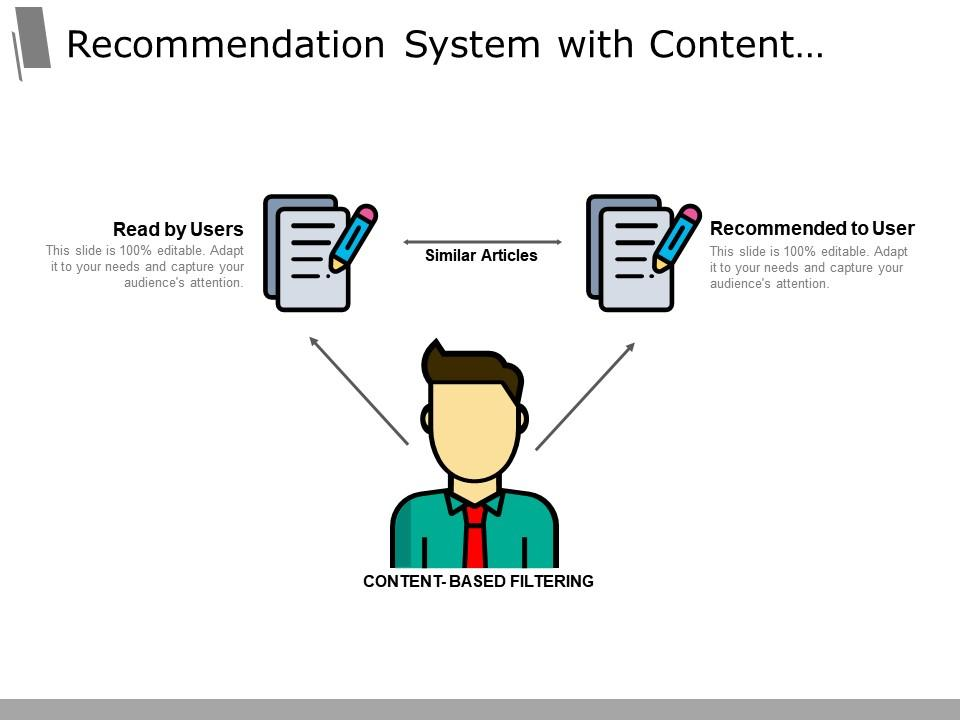
\includegraphics[width=0.8\textwidth]{pic/2}
    \label{fig:img1}
  \end{figure}  
\end{frame}

\begin{frame}{Коллаборативная фильтрация}
  \begin{figure}[H]
    \centering
    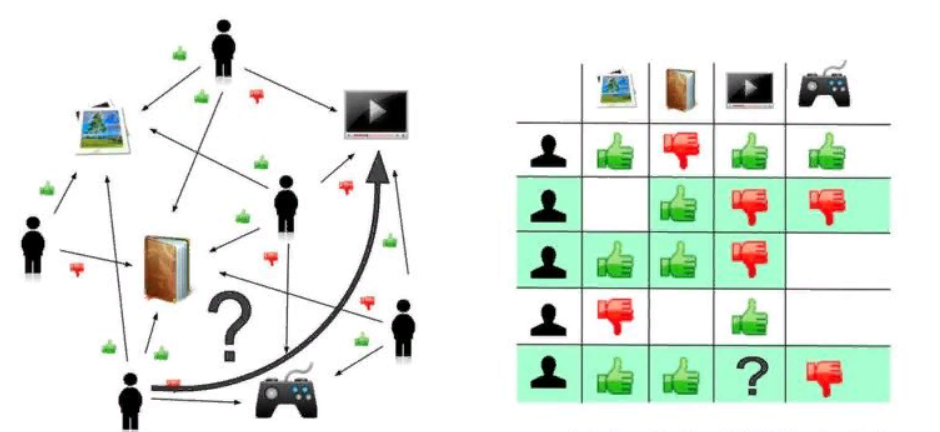
\includegraphics[width=0.8\textwidth]{pic/3}
    \label{fig:img1}
  \end{figure}  
\end{frame}

\begin{frame}{Гибридная фильтрация}
  \begin{figure}[H]
    \centering
    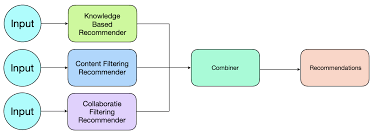
\includegraphics[width=0.7\textwidth]{pic/4}
    \label{fig:img1}
  \end{figure}  
\end{frame}

\begin{frame}
  \begin{center}
    {\Huge \textbf{Практическая часть}}
  \end{center}  
\end{frame}

\begin{frame}{Описание набора данных}
  В качестве основной выборки были использованы данные, предоставленные компанией H\&M для kaggle соревнования по построению рекомендательной системы. Данная выборка
  представляет из себя три таблицы, записанные в формате CSV: таблицу пользователей (customres.csv), содержащую в себе признаки 1371980 пользователей, таблицу объектов (articles.csv),
  содержащую в себе признаки 105542 товаров магазина, и таблицу взаимодействий (transactions.csv), содержащую в себе факты покупки товаров пользователями.  
\end{frame}

\begin{frame}{Анализ данных}
  ???
\end{frame}

\begin{frame}{Используемые модели}
  В качестве бейзлайн модели была взята рекомендация популярного, который дальше был модифицирован с помощью нескольких простых правил:
  рекомендации популярного относительно целевой группы пользователя и его пола.

  В качестве модели, основанной на контенте была взята модель tf-idf из библиотеки implicit.

  Для матричного разложения были использованы модели ALS из библиотеки implicit и LightFM из одноименной библиотеки.
  Причем LightFM может также являться гибридной, так как это разложение может учитывать признаки пользователей и объектов. 
\end{frame}

\begin{frame}{Результаты обучения}
  В качестве целевой метрики была выбрана метрика MAP$@12$, так как данная метрика является целевой в данном соревнование.

  \begin{equation}
    \text{p}@k = \frac{\text{количество релевантных элементов}}{k}.
  \end{equation}
  \begin{equation}
    \text{ap}@k = \frac{1}{k}\sum_{i=1}^{k}r_i\text{p}@i,
  \end{equation}
  где $r_i$ принимает значение 1, в случае если $i$ элемент топа является релевантным, и 0 в обратном случае.
  \begin{equation}
    \text{map}@k = \frac{1}{n}\sum_{i=1}^{n}\text{ap}@k_j.
  \end{equation}
\end{frame}

\begin{frame}{Результаты обучения}
  Валидация моделей проводилась на последней неделе тренировочной выборки. А в качестве тестовой использовались закрытые данные,
  на которых тестовая система соревнования оценивает качество прогноза моделей. Которая в свою очередь поделена на две части в
  соотношении 1 к 99. Ее наименьшая часть называется public, а наибольшая "--- private, за счет чего можно сравнить скорость
  деградации моделей.

  Результаты обучения моделей приведены в таблице 1.
\end{frame}

\begin{frame}{Результаты обучения}
  \begin{figure}[H]
    \centering
    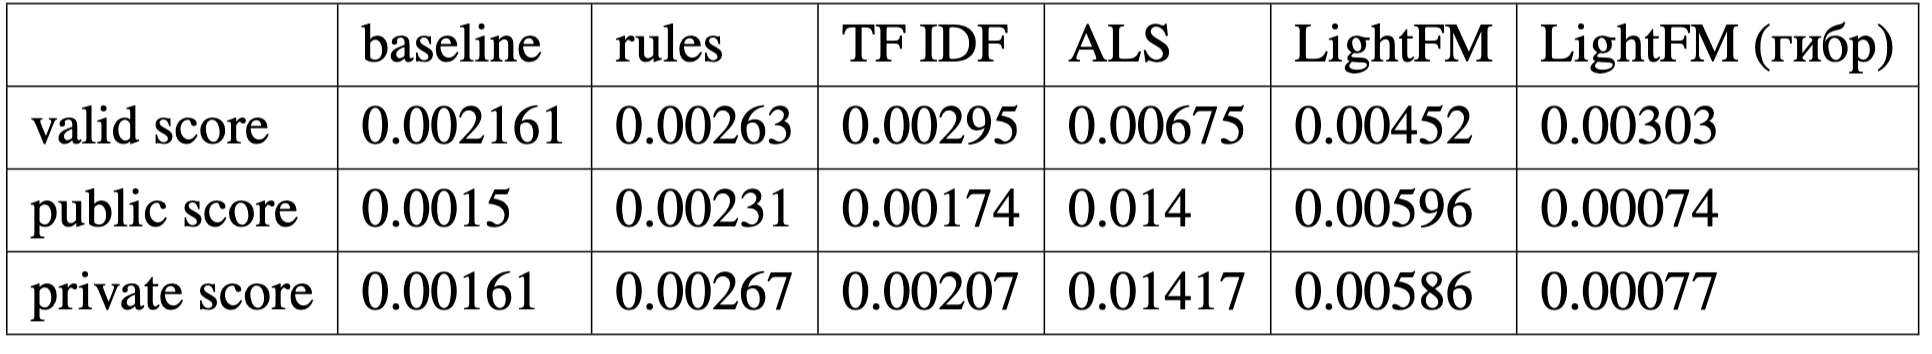
\includegraphics[width=1.\textwidth]{pic/5}
    \label{fig:img1}
  \end{figure}
\end{frame}

\begin{frame}{Выводы}
  По результатам, которые выдали модели можно сделать следующие выводы:
\begin{enumerate}
    \item Модели, основанные на рекомендации популярного очень быстро деградируют, однако этот минус нивелируется
    тем, что их не нужно обучать. Достаточно просто рассчитывать, какие товары находятся в тренде в данный момент времени
    с помощью одного запроса в базу данных.
    \item Усложнив запрос в базу данных несколькими простыми правилами, можно сильно поднять качество бейзлайна.
    \item Модели матричной факторизации дают лучшие метрики относительно любых моделей первого уровня, однако работают плохо
    с холодными пользователями и объектами.
    \item Гибридные модели первого уровня показывают себя намного хуже, чем любые другие модели первого уровня, при этом усложняя
    программную реализацию и расходуют больше времени на обучение.
\end{enumerate}
\end{frame}

\begin{frame}
  \frametitle{Внимание!}

  \begin{center}
    {\Huge \textbf{Спасибо за внимание!}}
  \end{center}
\end{frame}

\end{document}
